\documentclass[12pt]{article}

\usepackage{graphicx}
\usepackage{geometry}   %设置页边距的宏包
\usepackage{algpseudocode}
\usepackage{comment}
\usepackage{amsmath, amssymb, amsthm, mathdots}
\usepackage{enumerate}
\usepackage{enumitem}
\usepackage{framed}
\usepackage{verbatim}
\usepackage{microtype}
\usepackage{kpfonts}
\usepackage{multicol}
\usepackage{amsfonts}
\usepackage{array}
\usepackage{color}
\usepackage{graphicx}
\graphicspath{ {./image/} }
\newcommand{\solu}{{\color{blue} Solution:}}
\newcommand{\overbar}[1]{\mkern 1.5mu\overline{\mkern-1.5mu#1\mkern-1.5mu}\mkern 1.5mu}
\newcommand{\Ib}{\mathbf{I}}
\newcommand{\Pb}{\mathbf{P}}
\newcommand{\Qb}{\mathbf{Q}}
\newcommand{\Rbf}{\mathbf{R}}
\newcommand{\Rbb}{\mathbb{R}}
\newcommand{\Nb}{\mathbf{N}}
\newcommand{\Fb}{\mathbf{F}}
\newcommand{\Z}{\mathbf{Z}}
\newcommand{\Lap}{\mathcal{L}}
\newcommand{\Zplus}{\mathbf{Z}^+}
\newcommand{\Ubf}{\mathbf{U}}
\newcommand{\Upmb}{\pmb{U}}
\newcommand{\Ipmb}{\mathbf{I}}
\geometry{left=1.5cm,right=1.5cm,top=1.5cm,bottom=2cm}  %设置 上、左、下、右 页边距

\title{DS4400 HW1}
\date{}
\author{Xin Guan}

\begin{document}
\maketitle
\begin{enumerate}
    \item Let $\pmb{a} \in \Rbb^n$ be an $n$-dimensional vector and let $\Upmb \in \Rbb^{n \times n}$ be an orthonormal matrix, i.e., $\Upmb^{T} \Upmb = \Upmb \Upmb^{T} = \Ipmb_n$. show the following:
          \begin{enumerate}
              \item trace($\pmb{a}\pmb{a}^T$) = $||\pmb{a}||^2_2$

                    \solu
                    \begin{proof}
                        Let $\pmb{a} = \begin{bmatrix}
                            a_1 \\ 
                            a_2 \\
                            \dots \\ 
                            a_n
                        \end{bmatrix}$

                        Then,
                        $
                            \pmb{a}\pmb{a}^T=
                            \begin{bmatrix}
                                a_{1}  \\
                                a_{2}  \\
                                \vdots \\
                                a_{n}
                            \end{bmatrix} \cdot
                            \begin{bmatrix}
                                a_{1} & a_2 & \cdots & a_n
                            \end{bmatrix}
                            =
                            \begin{bmatrix}
                                a_1 \cdot a_1 & a_1 \cdot a_2 & \dots  & a_1 \cdot a_n \\
                                a_2 \cdot a_1 & a_2 \cdot a_2 & \dots  & a_2 \cdot a_n \\
                                \vdots        & \ddots        &        & \vdots        \\
                                \vdots        &               & \ddots & \vdots        \\
                                a_n \cdot a_1 & a_n \cdot a_2 & \dots  & a_n \cdot a_n
                            \end{bmatrix}
                        $

                        Therefore, trace($\pmb{a}\pmb{a}^T$) = $a_1 \cdot a_1 + a_2 \cdot a_2 + \cdots + a_n \cdot a_n$ = $\sum_{i = 1}^{n} a_i^2$ = $||\pmb{a}||^2_2$

                        Thus, trace($\pmb{a}\pmb{a}^T$) = $||\pmb{a}||^2_2$
                    \end{proof}

              \item $||\Upmb \pmb{a}||_2^2$ = $||\pmb{a}||_2^2$

                    \solu
                    \begin{proof}

                        We can write $\Upmb$ as follow:

                        $
                            \Upmb =
                            \begin{bmatrix}
                                v_1 & v_2 & \dots & v_n
                            \end{bmatrix}
                        $, where $v_i \in \Rbb^n, i\in \Z, 1 \le i \le n$.

                        We can write $\pmb{a} = \begin{bmatrix}
                            a_1 \\ a_2 \\ \vdots \\ a_n
                        \end{bmatrix}$, where $a_i \in \Rbb, 1 \le i \le n$

                        Since $\Upmb$ is orthonormal, we have:\\
                        $\forall i \ne k, v_iv_k = \overrightarrow{\pmb{0}}$\\
                        $\forall i\in \Z, 1 \le i \le n, v_i^T v_i = 1$

                        Then, we can write $\Upmb\pmb{a} =
                            \begin{bmatrix}
                                v_1a_1 + v_2a_2 + \dots + v_na_n
                            \end{bmatrix}$

                        Therefore, $||\Upmb\pmb{a}||^2_2 = (v_1a_1)^2 + (v_2a_2)^2 + \dots + (v_na_n)^2 \\
                            = \sum_{i = 1}^n (v_i^Ta_i)^2 \\
                            = \sum_{i = 1}^n (v_ia_i)^T(v_ia_i) \\
                            = \sum_{i = 1}^n (a_iv_i^T)(v_ia_i) \\
                            = \sum_{i = 1}^n (a_i(v_i^Tv_i)a_i)$ \\
                        Since $\forall i\in \Z, 1 \le i \le n, v_i^T v_i = 1$, we have:\\
                        $\sum_{i = 1}^n (a_i(v_i^Tv_i)a_i) \\
                        = \sum_{i = 1}^n (a_ia_i) \\
                        = ||\pmb{a}||^2_2$

                        Thus, $||\Upmb \pmb{a}||_2^2$ = $||\pmb{a}||_2^2$.
                    \end{proof}
          \end{enumerate}

    \item Let $\pmb{A} \in \Rbb^{n\times n}$ and $\pmb{B} \in \Rbb^{n\times n}$ be arbitrary but invertible matrices and let $\alpha$ be a scalar. Show the following:

          \begin{enumerate}
              \item $(\pmb{A}\pmb{B})^{-1} = \pmb{B}^{-1}\pmb{A}^{-1}$

                    \solu

                    \begin{proof}
                        By the definition of inverse, we have: $$(\pmb{A}\pmb{B})(\pmb{A}\pmb{B})^{-1} = \pmb{I}_n$$
                        Multiply both sides by $\pmb{A}^{-1}$: $$\pmb{A}^{-1}\pmb{A}\pmb{B}(\pmb{A}\pmb{B})^{-1} = \pmb{A}^{-1}\pmb{I}_n$$
                        Then we have: $$\pmb{B}(\pmb{A}\pmb{B})^{-1} = \pmb{A}^{-1}$$
                        Multiply both sides by $\pmb{B}^{-1}$: $$\pmb{B}^{-1}\pmb{B}(\pmb{A}\pmb{B})^{-1} = \pmb{B}^{-1}\pmb{A}^{-1}$$
                        Then we have: $$(\pmb{A}\pmb{B})^{-1} = \pmb{B}^{-1}\pmb{A}^{-1}$$
                        Therefore, $(\pmb{A}\pmb{B})^{-1} = \pmb{B}^{-1}\pmb{A}^{-1}$
                    \end{proof}



              \item $(\pmb{A}^T)^{-1} = (\pmb{A}^{-1})^T$

                    \solu

                    \begin{proof}
                        By the definition of inverse, we have $\pmb{A}^{-1}\pmb{A} = \pmb{I}_n$. Then we transpose both sides:
                        $$(\pmb{A}^{-1}\pmb{A})^T = (\pmb{I}_n)^T$$
                        Then we have: $$\pmb{A}^T(\pmb{A}^{-1})^T = \pmb{I}_n$$
                        Multiply both sides by $(\pmb{A}^T)^{-1}$:
                        $$(\pmb{A}^T)^{-1}\pmb{A}^T(\pmb{A}^{-1})^T = (\pmb{A}^T)^{-1}\pmb{I}_n$$
                        Then we have: $$(\pmb{A}^{-1})^T = (\pmb{A}^T)^{-1}$$
                    \end{proof}

              \item trace($\alpha \pmb{A}) = \alpha$ trace($\pmb{A}$)

                    \solu 
                    \begin{proof}
                        Let $\pmb{A} = \begin{bmatrix}
                            a_{11} & a_{12} & \dots & a_{1n}\\
                            a_{21} & a_{22} & \dots & a_{2n}\\
                            \vdots & \ddots &  & \vdots\\
                            a_{11} & a_{12} & \dots & a_{1n}
                        \end{bmatrix}$\\
                        Then $\alpha\pmb{A} = \begin{bmatrix}
                            \alpha a_{11} & \alpha a_{12} & \dots & \alpha a_{1n}\\
                            \alpha a_{21} & \alpha a_{22} & \dots & \alpha a_{2n}\\
                            \vdots & \ddots &  & \vdots\\
                            \alpha a_{11} & \alpha a_{12} & \dots & \alpha a_{nn}
                        \end{bmatrix}$\\
                        Then, trace($\alpha\pmb{A}$) = $\alpha a_{11} + \alpha a_{22} + \dots \alpha a_{nn} = \sum_{i = 1}^n \alpha a_{ii} = \alpha\sum_{i = 1}^n  a_{ii}$\\
                        On the other hand, $\alpha$ trace($\pmb{A}$) = $\alpha \cdot (a_{11} + a_{22} + \dots a_{nn}) = \alpha\sum_{i = 1}^n  a_{ii}$

                        Therefore, trace($\alpha \pmb{A}) = \alpha$ trace($\pmb{A}$)
                    \end{proof}
                    
                    
          \end{enumerate}
          \item For vectors $\pmb{x} \in \Rbb^n, \pmb{a} \in \Rbb^n$ and matrices $\pmb{X}\in \Rbb^{n \times n}, \pmb{A} \in \Rbb^{n \times n}$, show the following:
          \begin{enumerate}
            \item $\frac{\partial \pmb{a}^T\pmb{Ax}}{\partial \pmb{x}} = \pmb{A}^T\pmb{a}$
            
            \solu 

            We write $\pmb{A}$ as follow: 
            $\pmb{A} = \begin{bmatrix}
                v_1 & v_2 & \dots & v_n \\
            \end{bmatrix}$, where $v_i \in \Rbb^n, \forall i \in \Z, 1\le i \le n$

            Then $\pmb{a}^T\pmb{A} = 
            \begin{bmatrix}
                \pmb{a}^Tv_1 & \pmb{a}^Tv_2 & \dots &\pmb{a}^Tv_n
            \end{bmatrix}$

            We write $\pmb{x}$ as follow:
            $\begin{bmatrix}
                x_1 \\
                x_2 \\
                \dots \\
                x_n
            \end{bmatrix}$, where $x_i \in \Rbb, \forall i \in \Z, 1\le i \le n$

            Then $\pmb{a}^T\pmb{Ax} = 
                \pmb{a}^Tv_1x_1 + \pmb{a}^Tv_2x_2 + \dots + \pmb{a}^Tv_nx_n$

            Then, on the left hand side: $\frac{\partial \pmb{a}^T\pmb{Ax}}{\partial \pmb{x}} = 
            \begin{bmatrix}
                \pmb{a}^Tv_1 \\ \pmb{a}^Tv_2 \\ \dots \\ \pmb{a}^Tv_n
            \end{bmatrix}$

            On the right hand side: $\pmb{A}^T\pmb{a} = \begin{bmatrix}
                v_1^T \\
                v_2^T \\
                \dots \\
                v_n^T \\
            \end{bmatrix} \pmb{a} =
            \begin{bmatrix}
                v_1^T\pmb{a} \\
                v_2^T\pmb{a} \\
                \dots \\
                v_n^T\pmb{a}
            \end{bmatrix} = 
            \begin{bmatrix}
                \pmb{a}^Tv_1 \\ \pmb{a}^Tv_2 \\ \dots \\ \pmb{a}^Tv_n
            \end{bmatrix}
            $

            Therefore, $\frac{\partial \pmb{a}^T\pmb{Ax}}{\partial \pmb{x}} = \pmb{A}^T\pmb{a}$
            
            \item $\frac{\partial trace(\pmb{A}^T\pmb{X})}{\partial \pmb{X}} = \pmb{A}$ 
            
            \solu 

            we write $\pmb{A} = \begin{bmatrix}
                a_{11} & a_{12} & \dots & a_{1n} \\
                a_{21} & a_{22} & \dots & a_{2n} \\
                \vdots & \ddots &  & \vdots \\
                a_{n1} & a_{n2} & \dots & a_{nn}
            \end{bmatrix}, \pmb{X} = 
            \begin{bmatrix}
                x_{11} & x_{12} & \dots & x_{1n} \\
                x_{21} & x_{22} & \dots & x_{2n} \\
                \vdots & \ddots &  & \vdots \\
                x_{n1} & x_{n2} & \dots & x_{nn}
            \end{bmatrix}$\\
            Then, $\pmb{A}^T\pmb{X} = 
            \begin{bmatrix}
                \sum_{i = 1}^n a_{i1}x_{i1} & \sum_{i = 1}^n a_{i1}x_{i2} & \dots & \sum_{i = 1}^n a_{i1}x_{in}\\
                \sum_{i = 1}^n a_{i2}x_{i1} & \sum_{i = 1}^n a_{i2}x_{i2} & \dots & \sum_{i = 1}^n a_{i2}x_{in} \\
                \vdots & \ddots &  & \vdots \\
                \sum_{i = 1}^n a_{in}x_{i1} & \sum_{i = 1}^n a_{in}x_{i2}& \dots  &  \sum_{i = 1}^n a_{in}x_{in}
            \end{bmatrix}$\\
            trace$(\pmb{A}^T\pmb{X}) = \sum_{i = 1}^n a_{i1}x_{i1} + \sum_{i = 1}^n a_{i2}x_{i2}  + \dots \sum_{i = 1}^n a_{in}x_{in} \\
            = \sum_{j = 1}^{n}\sum_{i = 1}^{n} a_{ij}x_{ij}$

            Then, $\frac{\partial trace(\pmb{A}^T\pmb{X})}{\partial \pmb{X}} =
            \begin{bmatrix}
                a_{11} & a_{12} & \dots & a_{1n} \\
                a_{21} & a_{22} & \dots & a_{2n} \\
                \vdots & \ddots &  & \vdots \\
                a_{n1} & a_{n2} & \dots & a_{nn} \\
            \end{bmatrix} = \pmb{A}
            $ 

            Therefore, $\frac{\partial trace(\pmb{A}^T\pmb{X})}{\partial \pmb{X}} = \pmb{A}$ 
            
            \item $\frac{\partial ||\pmb{Ax}||^2_2}{\partial x} = 2\pmb{A}^T \pmb{A}\pmb{x}$
            
            \solu 

            we write $\pmb{A}$ as $\begin{bmatrix}
                a_{11} & a_{12} & \dots & a_{1n} \\
                a_{21} & a_{22} & \dots & a_{2n} \\
                \vdots & \ddots &  & \vdots \\
                a_{n1} & a_{n2} & \dots & a_{nn} \\
            \end{bmatrix}$,

            $x \text{ as } \begin{bmatrix}
                x_1 \\ x_2 \\ \dots \\ x_n
            \end{bmatrix}$

            Then $||\pmb{Ax}|| = \begin{bmatrix}
                a_{11}x_1 + a_{12}x_2 + \dots + a_{1n}x_n \\
                a_{21}x_1 + a_{22}x_2 + \dots + a_{2n}x_n \\
                \dots \\
                a_{n1}x_1 + a_{n2}x_2 + \dots + a_{nn}x_n \\
            \end{bmatrix}$

            Then $||Ax||^2_2 \\
            = (a_{11}x_1 + a_{12}x_2 + \dots + a_{1n}x_n)^2 + (a_{21}x_1 + a_{22}x_2 + \dots + a_{2n}x_n)^2 + \dots + (a_{n1}x_1 + a_{n2}x_2 + \dots + a_{nn}x_n)^2 \\
            = (\sum_{i = 1}^n a_{1i}x_i)^2 + (\sum_{i = 1}^n a_{2i}x_i)^2 \dots + (\sum_{i = 1}^n a_{ni}x_i)^2 \\$

            Then on the left hand side: \\
            $$\frac{\partial ||\pmb{Ax}||^2}{\partial x} $$
            $$= \frac{\partial [(\sum_{i = 1}^n a_{1i}x_i)^2 + (\sum_{i = 1}^n a_{2i}x_i)^2 \dots + (\sum_{i = 1}^n a_{ni}x_i)^2 ]}{\partial x} $$
            $$= \frac{\partial (\sum_{i = 1}^n a_{1i}x_i)^2}{\partial x} + \frac{\partial (\sum_{i = 1}^n a_{2i}x_i)^2}{\partial x} + \dots + \frac{\partial (\sum_{i = 1}^n a_{ni}x_i)^2}{\partial x} $$
            $$= 2(\sum_{i = 1}^n a_{1i}x_i)\frac{\partial (\sum_{i = 1}^n a_{1i}x_i)}{\partial x} + 2(\sum_{i = 1}^n a_{2i}x_i)\frac{\partial (\sum_{i = 1}^n a_{2i}x_i)}{\partial x} + \dots + 2(\sum_{i = 1}^n a_{ni}x_i)\frac{\partial (\sum_{i = 1}^n a_{ni}x_i)}{\partial x} $$
            $$= 2(\sum_{i = 1}^n a_{1i}x_i)\begin{bmatrix}
                a_{11}\\ a_{12} \\ \dots \\ a_{1n}
            \end{bmatrix} + 
            2(\sum_{i = 1}^n a_{2i}x_i)\begin{bmatrix}
                a_{21}\\ a_{22} \\ \dots \\ a_{2n}
            \end{bmatrix} + \dots + 
            2(\sum_{i = 1}^n a_{ni}x_i)\begin{bmatrix}
                a_{n1}\\ a_{n2} \\ \dots \\ a_{nn}
            \end{bmatrix} $$
            $$= 2 \begin{bmatrix}
                (\sum_{i = 1}^n a_{1i}x_i) a_{11} + (\sum_{i = 1}^n a_{2i}x_i) a_{21} + \dots + (\sum_{i = 1}^n a_{ni}x_i) a_{n1} \\
                (\sum_{i = 1}^n a_{1i}x_i) a_{12} + (\sum_{i = 1}^n a_{2i}x_i) a_{22} + \dots + (\sum_{i = 1}^n a_{ni}x_i) a_{n2} \\
                \vdots \\
                (\sum_{i = 1}^n a_{1i}x_i) a_{1n} + (\sum_{i = 1}^n a_{2i}x_i) a_{2n} + \dots + (\sum_{i = 1}^n a_{ni}x_i) a_{nn} \\
            \end{bmatrix} \\$$
            On right hand side: \\
            $$2\pmb{A^TAx} = 2\pmb{A^T}(\pmb{Ax})$$
            $$= 2\begin{bmatrix}
                a_{11} & a_{21} & \dots & a_{n1} \\
                a_{12} & a_{22} & \dots & a_{n2} \\
                \vdots & \ddots &  & \vdots \\
                a_{1n} & a_{2n} & \dots & a_{nn} \\
            \end{bmatrix}
            \begin{bmatrix}
                a_{11}x_1 + a_{12}x_2 + \dots + a_{1n}x_n \\
                a_{21}x_1 + a_{22}x_2 + \dots + a_{2n}x_n \\
                \dots \\
                a_{n1}x_1 + a_{n2}x_2 + \dots + a_{nn}x_n \\
            \end{bmatrix} $$
            $$= 2\begin{bmatrix}
                a_{11} & a_{21} & \dots & a_{n1} \\
                a_{12} & a_{22} & \dots & a_{n2} \\
                \vdots & \ddots &  & \vdots \\
                a_{1n} & a_{2n} & \dots & a_{nn} \\
            \end{bmatrix}
            \begin{bmatrix}
                \sum_{i = 1}^n a_{1i}x_i \\
                \sum_{i = 1}^n a_{2i}x_i  \\
                \dots \\
                \sum_{i = 1}^n a_{ni}x_i \\
            \end{bmatrix} $$
            $$= 2\begin{bmatrix}
                (\sum_{i = 1}^n a_{1i}x_i)\cdot a_{11} + (\sum_{i = 1}^n a_{2i}x_i)\cdot a_{21} + \dots + (\sum_{i = 1}^n a_{ni}x_i)\cdot a_{n1} \\
                (\sum_{i = 1}^n a_{1i}x_i)\cdot a_{12} + (\sum_{i = 1}^n a_{2i}x_i)\cdot a_{22} + \dots + (\sum_{i = 1}^n a_{ni}x_i)\cdot a_{n2} \\
                \vdots \\
                (\sum_{i = 1}^n a_{1i}x_i)\cdot a_{1n} + (\sum_{i = 1}^n a_{2i}x_i)\cdot a_{2n} + \dots + (\sum_{i = 1}^n a_{ni}x_i)\cdot a_{nn}
            \end{bmatrix}$$

            % = 2\begin{bmatrix}
            %     (\sum_{i = 1}^{n} a_{i1}a_{i1})x_1 + (\sum_{i = 1}^{n} a_{i2}a_{i1})x_2 + \dots + (\sum_{i = 1}^{n} a_{in}a_{i1})x_n \\
            %     (\sum_{i = 1}^{n} a_{i1}a_{i2})x_1 + (\sum_{i = 1}^{n} a_{i2}a_{i2})x_2 + \dots + (\sum_{i = 1}^{n} a_{in}a_{i2})x_n \\
            %     \dots \\
            %     (\sum_{i = 1}^{n} a_{i1}a_{in})x_1 + (\sum_{i = 1}^{n} a_{i2}a_{in})x_2 + \dots + (\sum_{i = 1}^{n} a_{in}a_{in})x_n \\
            % \end{bmatrix}$

            % If we write $\pmb{A}$ as $\begin{bmatrix}
            %     v_1 & v_2 & \dots & v_n
            % \end{bmatrix}$ 
            
            % where $v_i = \begin{bmatrix}
            %     a_{1i} \\ a_{2i} \\ a_{3i} \\ \dots \\ a_{ni}
            % \end{bmatrix}$

            % Then we can write the expression above as $2\begin{bmatrix}
            %     v_1^T v_1 x_1 + v_2^T v_1 x_2 + \dots v_n^T v_1 x_n \\
            %     v_1^T v_2 x_1 + v_2^T v_2 x_2 + \dots v_n^T v_2 x_n \\
            %     \dots \\
            %     v_1^T v_n x_1 + v_2^T v_n x_2 + \dots v_n^T v_n x_n \\
            % \end{bmatrix}$

            % Therefore, $\frac{\partial ||\pmb{Ax}||^2}{\partial x} =2\begin{bmatrix}
            %     v_1^T v_1 x_1 + v_2^T v_1 x_2 + \dots v_n^T v_1 x_n \\
            %     v_1^T v_2 x_1 + v_2^T v_2 x_2 + \dots v_n^T v_2 x_n \\
            %     \dots \\
            %     v_1^T v_n x_1 + v_2^T v_n x_2 + \dots v_n^T v_n x_n \\
            % \end{bmatrix}$

            % on the right hand side: $2\pmb{A}^T \pmb{A}\pmb{x} = 2
            % \begin{bmatrix}
            %     v_1 & v_2 & \dots & v_n
            % \end{bmatrix}^T
            % \begin{bmatrix}
            %     v_1 & v_2 & \dots & v_n
            % \end{bmatrix}
            % \begin{bmatrix}
            %     x_1 \\ x_2 \\ \dots \\ x_n
            % \end{bmatrix} \\
            % = 2
            % \begin{bmatrix}
            %     v_1^T \\ v_2^T \\ \dots \\ v_n^T
            % \end{bmatrix}
            % \begin{bmatrix}
            %     v_1 & v_2 & \dots & v_n
            % \end{bmatrix}
            % \begin{bmatrix}
            %     x_1 \\ x_2 \\ \dots \\ x_n
            % \end{bmatrix}\\
            % = 2 \begin{bmatrix}
            %     v_1^Tv_1 & v_1^Tv_2 & \dots & v_1^Tv_n \\
            %     v_2^Tv_1 & v_2^Tv_2 & \dots & v_2^Tv_n \\
            %     \vdots & \cdots & \cdots & \vdots\\
            %     v_n^Tv_1 & v_n^Tv_2 & \dots & v_n^Tv_n \\
            % \end{bmatrix}
            % \begin{bmatrix}
            %     x_1 \\ x_2 \\ \dots \\ x_n
            % \end{bmatrix}\\
            % = 2 \begin{bmatrix}
            %     v_1^Tv_1x_1 & v_1^Tv_2x_2 & \dots & v_1^Tv_nx_n \\
            %     v_2^Tv_1x_1 & v_2^Tv_2x_2 & \dots & v_2^Tv_nx_n \\
            %     \vdots & \cdots & \cdots & \vdots\\
            %     v_n^Tv_1x_1 & v_n^Tv_2x_2 & \dots & v_n^Tv_nx_n \\
            % \end{bmatrix}\\
            % = 2 \begin{bmatrix}
            %     v_1^Tv_1x_1 & v_2^Tv_1x_2 & \dots & v_n^Tv_1x_n \\
            %     v_1^Tv_2x_1 & v_2^Tv_2x_2 & \dots & v_n^Tv_2x_n \\
            %     \vdots & \cdots & \cdots & \vdots\\
            %     v_1^Tv_nx_1 & v_2^Tv_nx_2 & \dots & v_n^Tv_nx_n \\
            % \end{bmatrix}$
            
            Thus, left part equals right part.

            Therefore, $\frac{\partial ||\pmb{Ax}||^2_2}{\partial x} = 2\pmb{A}^T \pmb{A}\pmb{x}$
          \end{enumerate}

          \item Determine whether each of the following functions is convex or not.
          \begin{enumerate}
            \item $f(x) = (x-a)^2$, for any real number $a$.
              
            \solu

            Since this function is $\mathbb{R} \Rightarrow \mathbb{R}$, we can calculate its second order derivative to determine whether it is convex.

            $f'(x) = 2(x - a)$ \\
            $f''(x) = 2 \ge 0$

            Therefore, $f(x) = (x-a)^2$ is convex.

            \item $f(x) = -log(2x)$, with the domain $x \in (0,+\infty)$.
              
            \solu

            Since this function is $\mathbb{R} \Rightarrow \mathbb{R}$, we can calculate its second order derivative to determine whether it is convex.

            $f'(x) = -\frac{1}{x}$\\
            $f''(x) = \frac{1}{x^2}$\\
            since $x \in (0, +\infty),  f''(x) \ge 0$

            Therefore, $f(x) = -log(2x)$ is convex.

            \item $f(x) = e^{g(x)}$, where $g(x)$ is convex.
              
            \solu
            
            Since this function is $\mathbb{R} \Rightarrow \mathbb{R}$, we can calculate its second order derivative to determine whether it is convex.

            $f'(x) = e^{g(x)}g'(x)$\\
            $f''(x) = e^{g(x)}[g'(x)]^2 + e^{g(x)}g''(x)$\\
            Since $g(x)$ is convex, $g''(x) \ge 0$.\\
            And $e^{g(x)}[g'(x)]^2 \ge 0$, $e^{g(x)} \ge 0$.\\
            Then, $e^{g(x)}[g'(x)]^2 + e^{g(x)}g''(x) \ge 0$
            
            Therefore, $f(x) = e^{g(x)}$ is convex.
              
          \end{enumerate}

          \item question 5
          

          \begin{enumerate}
              \item \solu 
              
              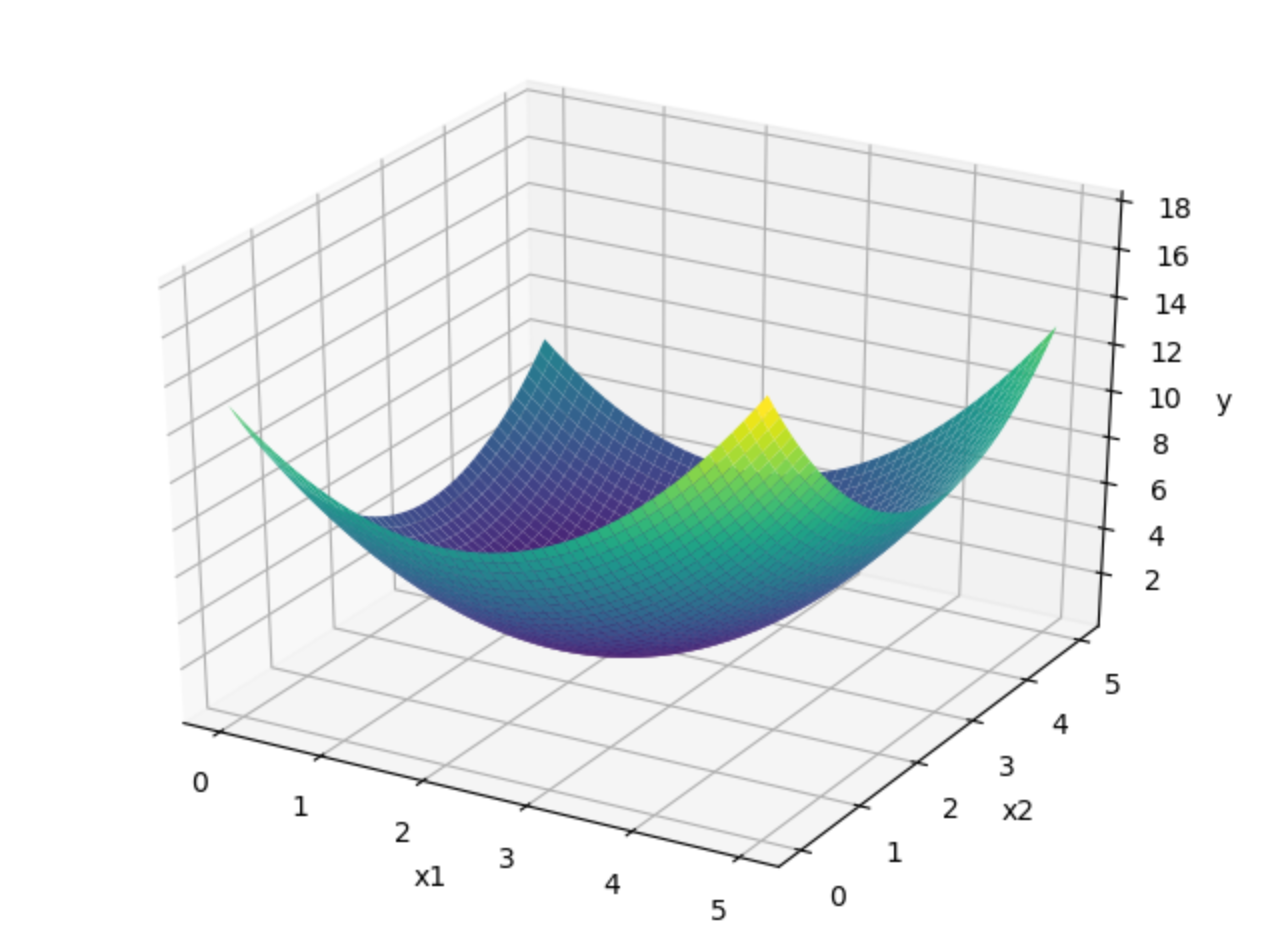
\includegraphics[scale=0.6]{q5plotfunction.png}

              \item \solu
              
              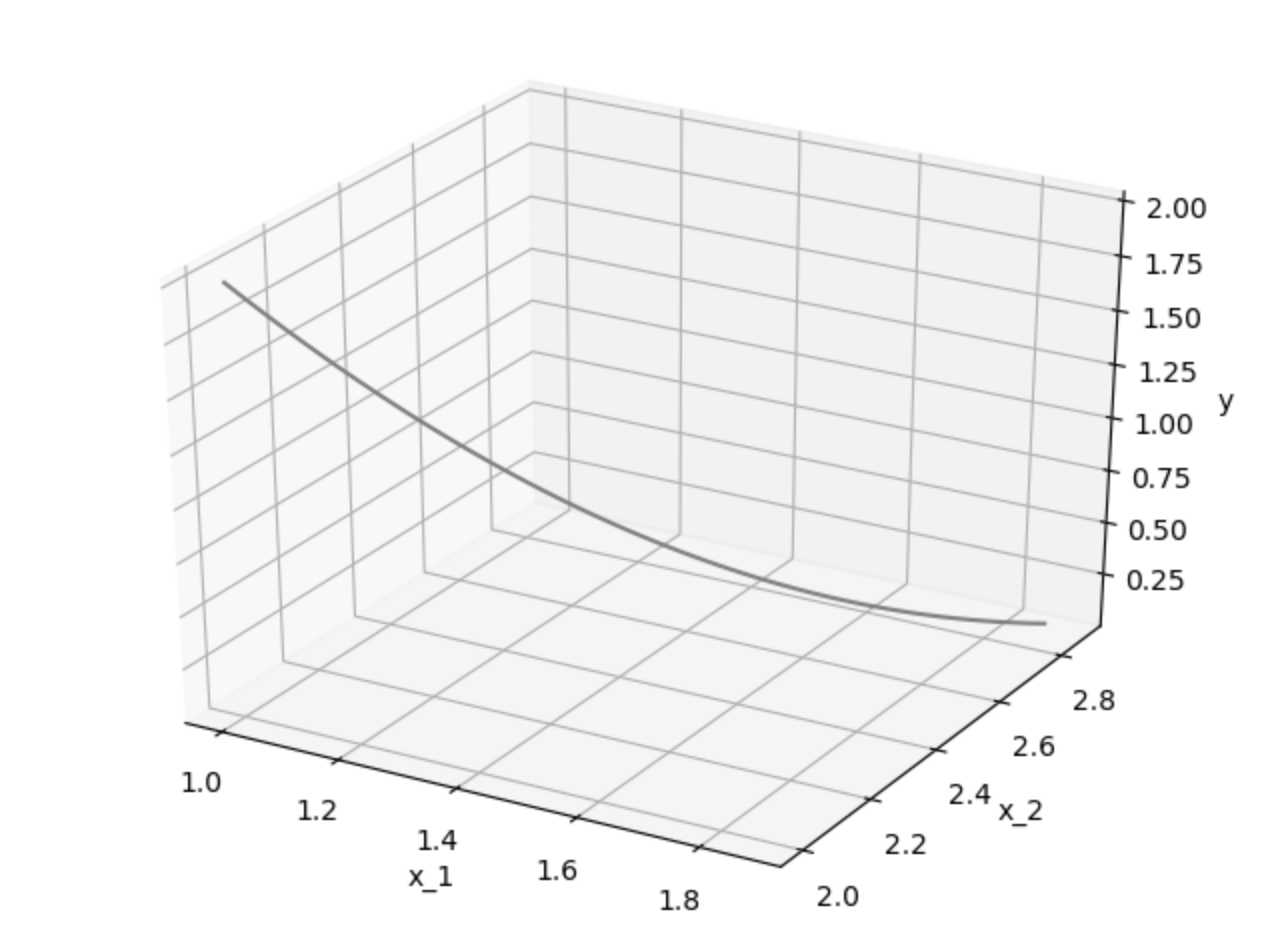
\includegraphics[scale=0.6]{q5_3.png}

              \item \solu
              
              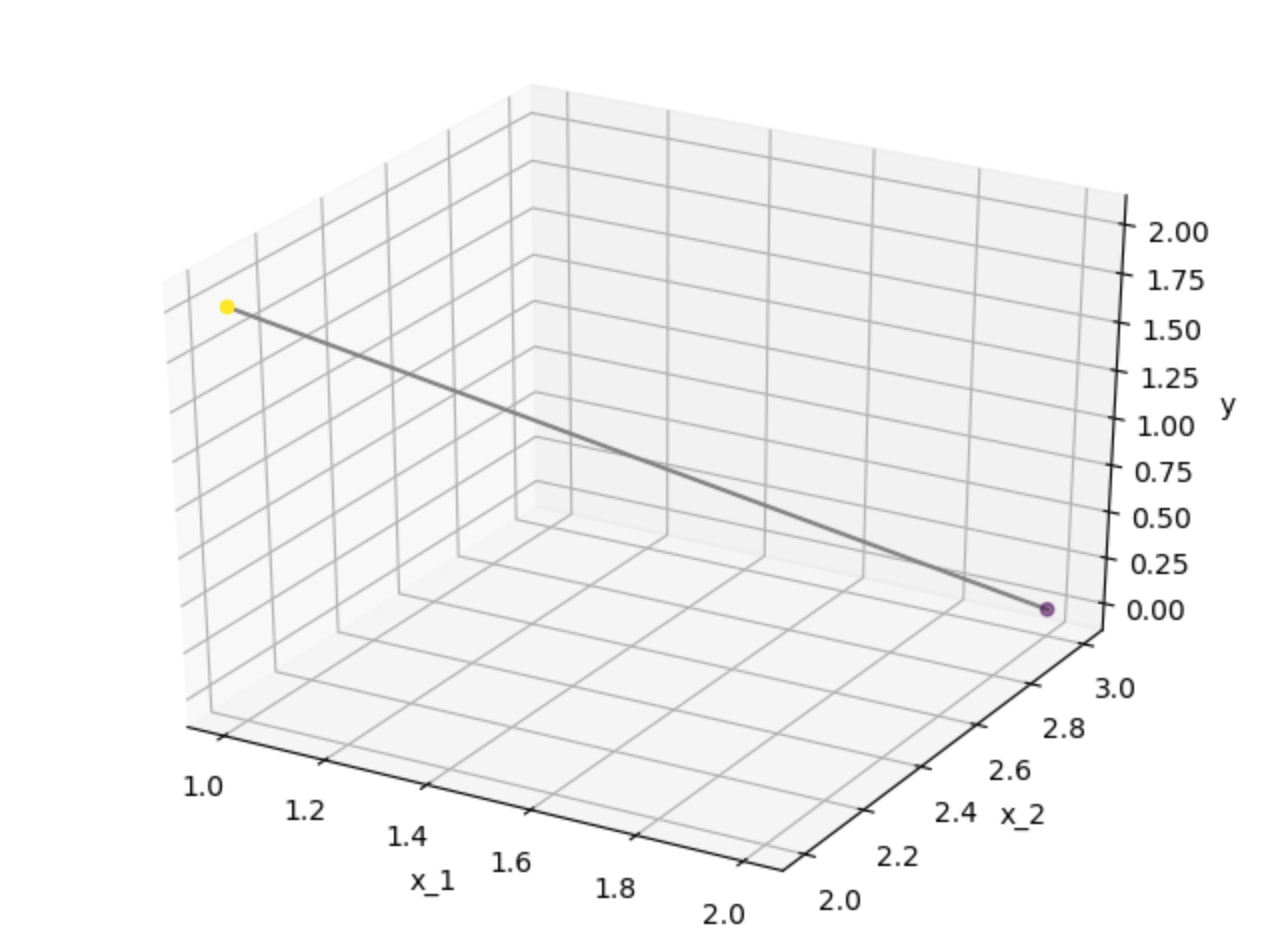
\includegraphics[scale=0.7]{q5_4.png}

              \item \solu
              
              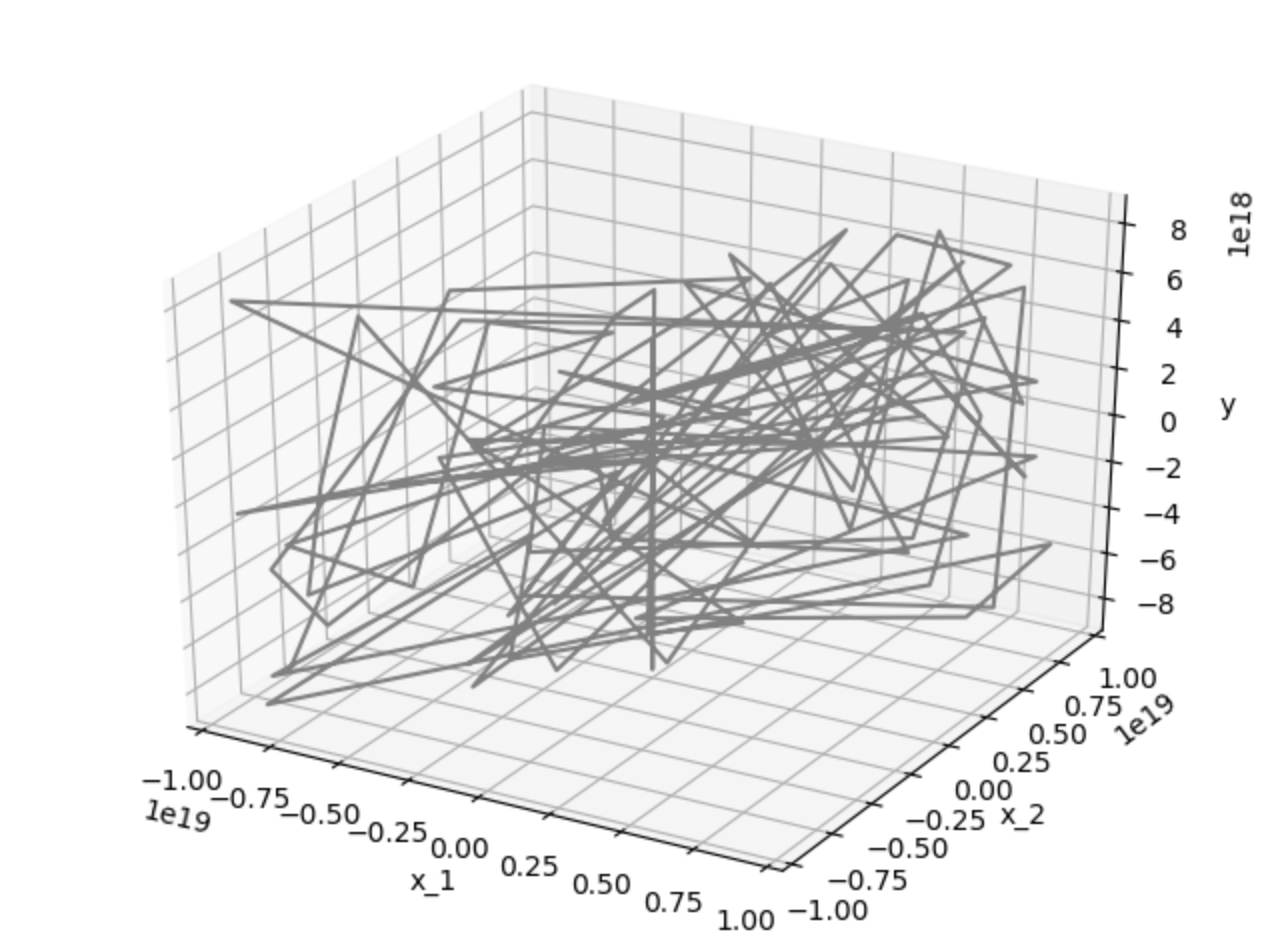
\includegraphics[scale=0.7]{q5_5.png}

          \end{enumerate}

          
          
          \item question 6
          
          \solu

          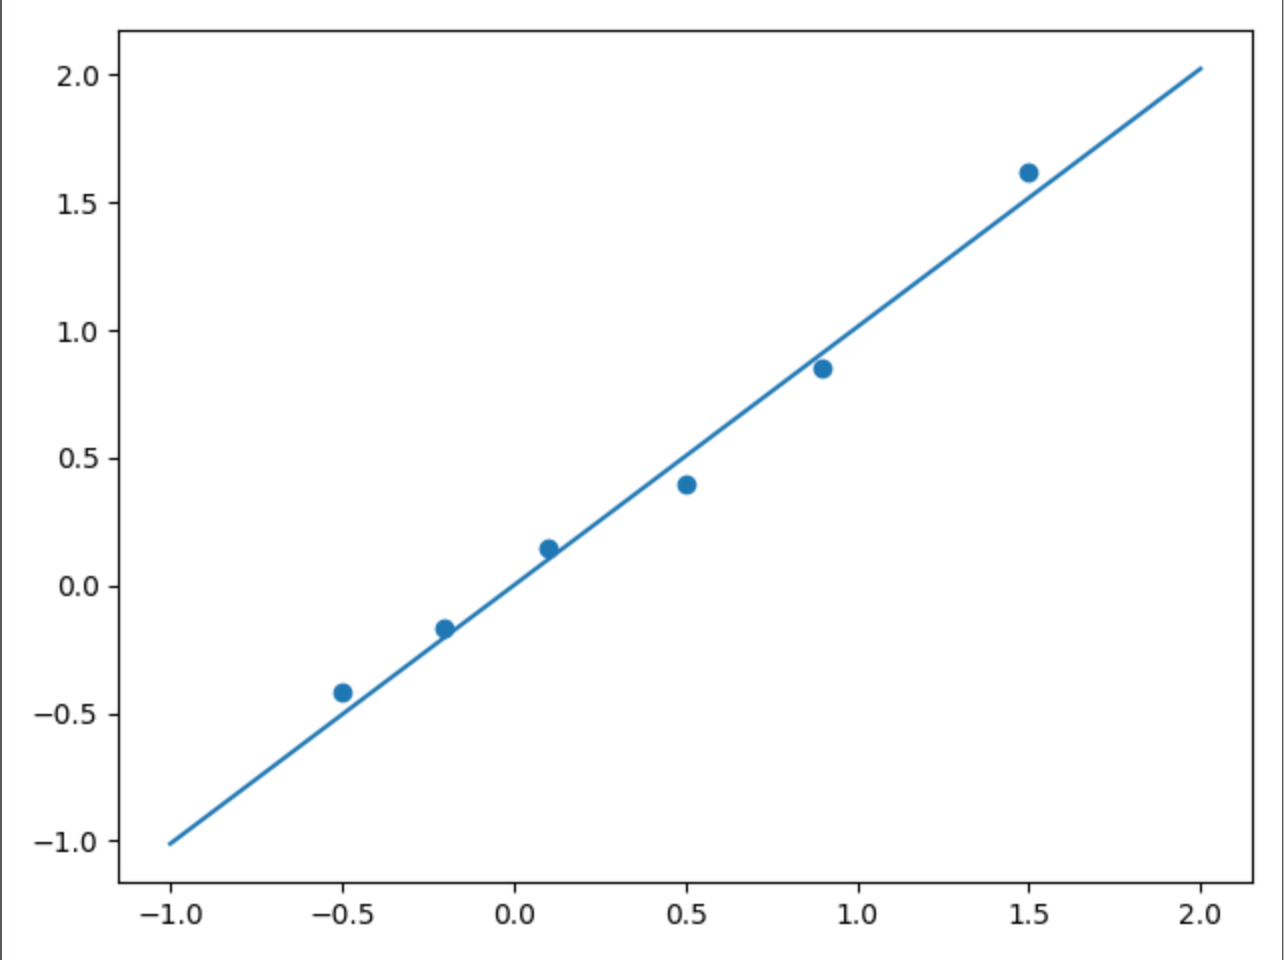
\includegraphics[scale=0.6]{q6.png}
          

\end{enumerate}
\end{document}